
%%%% ijcai17.tex

\typeout{Model-Free Conformant Planning}

% These are the instructions for authors for IJCAI-17.
% They are the same as the ones for IJCAI-11 with superficical wording
%   changes only.

\documentclass{article}
% The file ijcai17.sty is the style file for IJCAI-17 (same as ijcai07.sty).
\usepackage{ijcai17}

% Use the postscript times font!
\usepackage{times}

\usepackage{latexsym}
\usepackage{graphicx}
\usepackage{color}
\usepackage{multirow}
\usepackage{amsmath}
\usepackage{amssymb}
\usepackage{psfig}
\usepackage{subcaption}
\usepackage{tabularx}

\usepackage[ruled,vlined,linesnumbered]{algorithm2e}
\newtheorem{definition}{Definition}
\newtheorem{lemma}{Lemma}
\newtheorem{corollary}{Corollary}
% the following package is optional:
%\usepackage{latexsym} 

% Following comment is from ijcai97-submit.tex:
% The preparation of these files was supported by Schlumberger Palo Alto
% Research, AT\&T Bell Laboratories, and Morgan Kaufmann Publishers.
% Shirley Jowell, of Morgan Kaufmann Publishers, and Peter F.
% Patel-Schneider, of AT\&T Bell Laboratories collaborated on their
% preparation.

% These instructions can be modified and used in other conferences as long
% as credit to the authors and supporting agencies is retained, this notice
% is not changed, and further modification or reuse is not restricted.
% Neither Shirley Jowell nor Peter F. Patel-Schneider can be listed as
% contacts for providing assistance without their prior permission.

% To use for other conferences, change references to files and the
% conference appropriate and use other authors, contacts, publishers, and
% organizations.
% Also change the deadline and address for returning papers and the length and
% page charge instructions.
% Put where the files are available in the appropriate places.

\newenvironment{proof}{\noindent{\bf Proof:~~}}{\qed}
\newcommand{\tuple}[1]{\ensuremath{\left \langle #1 \right \rangle }}

\newcommand{\comment}[1]{}

\newcommand{\OPEN} {{\textsc{Open}}}

% This is for the agmin
\newcommand{\argmin}{\operatornamewithlimits{argmin}}


\newcommand{\ch}[1]
{{\color{red} #1}}

\newcommand{\qed}{\hfill\ensuremath{\blacksquare}}
\newcommand{\astar}{A$^*$}
\newcommand{\SAS}{SAS$^+$}
\newcommand{\wastar}{WA$^*$}
\newcommand{\arastar}{ARA$^*$}
\newcommand{\open}{\textsc{Open}}
\newcommand{\closed}{\textsc{Closed}}
\newcommand{\cmfp}{conformant model-free planning}
\newcommand{\eff}{\textit{eff}}
\newcommand{\pre}{\textit{pre}}
\newcommand{\solvable}{\textit{S}}
\newcommand{\plannable}{\textit{P}}
\newcommand{\true}{\textit{T}}
\newcommand{\false}{\textit{$\bot$}}


\setlength{\pdfpagewidth}{8.5in} \setlength{\pdfpageheight}{11in}
%\pdfinfo{
%/Title(To Reopen or Not to Reopen)
%/Author(Submission #85)}




\setcounter{secnumdepth}{2}
\newtheorem{theorem}{Theorem}

% Used for commenting
\newcommand{\commenter}[2]{\red{[\uppercase{#1}]:{#2}]}}
\newcommand{\roni}[1]{[[Roni:#1]]}
\newcommand{\brendan}[1]{\commenter{brendan}{#1}}



\newcommand{\MEMO}[1]
{ \fbox{
		\begin{minipage}[b]{7.9 cm}
			#1
		\end{minipage}
} }


\title{Model-Free Conformant Planning}
\author{Submission \#1365}

\begin{document}
	
	\maketitle
	
	\begin{abstract}
		In this paper we explore the theoretical boundaries of 
		conformant planning in a setting where 
		there is no model of the agent's actions. 
		Instead of an action model, a set of successfully executed plans are given and the task is to generate a plan that is guaranteed to achieve the goal without failing. 
		To this end we propose to learn a conservative model of the world, in which actions are guaranteed to be applicable. This conservative model is then given to an off-the-shelf classical planner, resulting in a plan that is guaranteed to achieve the goal. 
		Our reduction from a model-free planning problem to a model-based planning problem is sound but not complete, not finding plans even in cases when they exist. 
		Then, we analyze theoretically the probabilistic relation between the number of observed trajectories and the likelihood that our conservative approach will indeed fail to solve a solvable problem. Our analysis show that the number of trajectories needed scales gracefully.
	\end{abstract}
	
	\section{Introduction}
	% Planning problems
	In classical planning problems, a model of the acting agent and its relation to the relevant world is given in a formal planning description language, e.g., the classical STRIPS model~\cite{fikes1971strips} or PDDL~\cite{mcdermott1998pddl}. Planning algorithms (planners) use this model to generate a plan for achieving a given goal condition. 
	
	% Domain modeling is hard and so people try to automated this
	Creating a planning domain model for an agent, and in general knowledge engineering, is notoriously hard. %\roni{Brendan, if you have a nice reference for this?} 
	Thus, a well-studied approach is to learn a domain model by observing the agent's prior interactions with the environment, and by guiding the agent towards performing exploratory actions. A popular approach to planning without a domain model in {\em reinforcement learning} even skips the model-learning phase and directly learns how to act from observing the agent's past actions and observations~\cite[e.g.]{kearns2002}.  
	
	
	% We are different: only positive examples, and we really want to succeed
	In most prior work, the plans generated by the agent may fail, in which case the agent will replan, possibly refining an underlying domain model it has learned. Thus, the agent learns from both positive and negative examples. In this work we address a different setting, in which execution failure is very costly and must be avoided. Furthermore, an agent may have limited computational capabilities, and thus might not have the capability to re-plan after the plan it has tried to execute has failed. 
	Consider, for example, a team of nano-bots deployed inside a human body for medical target identification and drug delivery~\cite{cavalcanti2007nanorobot}. Re-planning is likely not possible in such nano-bots, and, of course, failing to cure the disease is undesirable. Thus, the planning task we focus on in this paper is how to find a plan that is guaranteed to achieve the goal, in a setting where a domain model is not available. We call this problem the {\em conformant model-free planning problem}. 
	
	
	% Our approach 
	First, we show how to learn a set of actions that the agent can use from the given trajectories. 
	For every such action $a$, we bound the set of predicates that are $a$'s preconditions and effects. This bounded action model is then used  to construct a conformant planning problem such that a solution to it is a solution to our model-free problem. This approach to solve the model-free planning problem 
	is sound and can be very efficient, since many conformant planning algorithms exist in the literature~\cite{palacios2009compiling,hoffmann2006conformant}. 
	However, it is not complete, as the conformant planning problem might not be solvable even if the underlying model-free planning problem is. Nonetheless, we prove that under some assumptions, the probability of this occurring decreases quasi-linearly with the number of observed trajectories. %\MEMO{I think it is better to say something more accurate than ``quickly''. How do you say in English taht something grows in a $n\cdot logn$ manner? super-linearly?}
	%We note that the contributionswhile the proposed solution this short paper lays the theoretical framework for model-free planning
	
	%In this paper we introduce a theoretical framework for learning a partial classical planning model from a given set of observed trajectories, and how to plan using these observed trajectoriesin a way that will ensure the goal is achieved. 
	
	
	%[[TAKEN FROM "Planning and Learning under Uncertainty" Ph.D. thesis of Sergio Jimenez Celorrio ]] In deterministic and totally observable environments this problem has been well studied. The LIVE system [92] learns operators with quantified variables while exploring the world. The EXPO system [45] refines incomplete planning operators when the monitoring of a plan execution detects a divergence between internal expectations and external observations. [98] learns PRODIGY operators from the execution traces of the resulting solutions or execution failures. The TRAIL system [6] limits its operators to an extended version of Horn clauses so that ILP can be applied. The LOPE system [41] proposed an integrated framework for learning, planning and executing actions
	
	
	
	\section{Problem Definition}
	The setting we address is a a STRIPS planning domain, represented 
	using the \SAS{} formalism~\cite{backstrom1995complexity}. 
	A planning domain in SAS$+$ is defined by the tuple $\mathcal{D}=\tuple{\mathcal{X}, \mathcal{O}}$, where 
	\begin{itemize}
		\item $\mathcal{X}=\{x_1,\ldots, x_n\}$ is a set of state variables, each associated with a finite domain $Dom(x_i)$. 
		\item $\mathcal{O}$ is a set of actions, where each action $a\in \mathcal{O}$      is defined by a tuple $\tuple{\pre(a), \eff(a)}$, where $\pre(a)$ and $\eff(a)$ are assignments of values to state variables, i.e., a set of assignments of the form $x_i=v$ where $v\in Dom(x_i)$. We refer to $\mathcal{O}$ and its associated sets of preconditions and effects as the {\em action model} of the domain.
	\end{itemize}
	
	A state is also a set of assignments of the form $x_i=v$ 
	such that every variable in $\mathcal{X}$ is assigned a single value from its corresponding domain. As a shorthand notation, if a state $s$ contains an assignment $x_i=v$ we will write $s(x_i)=v$. A planning problem in \SAS{} is defined by the tuple $\Pi=\tuple{\mathcal{D},s_\mathcal{I}, s_\mathcal{G}}$, where 
	$s_\mathcal{I}$ is the initial state and $s_\mathcal{G}$ 
	is a partial assignment of some state variables that defines the goal. A state $s$ is a goal state if $s_\mathcal{G}\subseteq s$. 
	For an action $a$ and a state $s$ we denote by $apply(s,a)$ the state
	resulting from applying $a$ on state $s$. 
	A solution to an \SAS{} planning problem is a {\em plan}, 
	which is a sequence of actions $a_1,\ldots,a_m$ such that  $s_\mathcal{G}\subseteq apply(\ldots apply(s,a_1), a_2)\ldots a_m)$. 
	
	%%%%% up to here
	The key challenge we address in this paper is how to solve a \SAS{} 
	planning problem $\Pi=\tuple{\mathcal{D},s_\mathcal{I}, s_\mathcal{G}}$ without having the action model of $\mathcal{D}$. Instead, a set of {\em trajectories} are assumed to be given. 
	\begin{definition}[Trajectory]
		A trajectory $T=\langle s_1, a_1, s_2, a_2, \ldots, a_{n-1}, s_n\rangle$ is an alternating sequence of states ($s_1,\ldots,s_n$) and actions ($a_1,\ldots,a_n$) that starts and ends with a state. 
	\end{definition}
	A trajectory represents a successful execution of a sequence of actions by the agent. A set of trajectories may be obtained, for example, by monitoring the acting agent when it is controlled manually by a human operator. The states in the given trajectories are assumed to be fully observable. 
	%\roni{Brendan, maybe we can think about what to do if we don't know the action names. Then, we can ``create'' actions, and maybe this will be more compact than the real actions? this can be pretty cool}
	
	Finally, we can define the {\em conformant model-free planning} problem, which is the focus of this work. 
	
	\begin{definition}[Conformant Model-free planning]
		Let $\Pi=\tuple{\tuple{\mathcal{X},\mathcal{O}},s_\mathcal{I}, s_\mathcal{G}}$ be a planning 
		problem and let $\mathcal{T}=\{\mathcal{T}^1,\ldots,\mathcal{T}^m\}$ be a set of trajectories in 
		the planning domain $\tuple{\mathcal{X},\mathcal{O}}$. 
		The input to a conformant model-free planning problem is 
		the tuple $\tuple{\mathcal{X},s_\mathcal{I}, s_\mathcal{G}, \mathcal{T}}$
		and the task is to generate a plan $\pi$  that is a solution to $\Pi$. We denote this conformant model-free planning problem as $\Pi_\mathcal{T}$. 
		\label{def:model-free-planning}
	\end{definition}
	
	%\begin{definition}[Conformant Model-free planning] The input to a conformant model-free planning problem is a tuple $\tuple{\mathcal{X},s_\mathcal{I}, s_\mathcal{G}, \mathcal{T}}$,  where $\mathcal{X}$, $s_\mathcal{I}$, and $s_\mathcal{G}$ are the state variables, initial state, and goal, respectively, of an underlying planning problem, and $\mathcal{T}$ is the given set of trajectories. The task is to generate plan that is a solution to the underlying planning problem, i.e.,  a a sequence of action that , if is applied to $s_\mathcal{I}$, will result in a state that satisfies $s_\mathcal{G}$. \label{def:model-free-planning}\end{definition}
	
	
	% 1!!!!!!!!!!!!!
	\section{Conservative Planning}
	%We follow Walsh and Litman's approach
	%We follow Wang's~\cite{wang1994learning,wang1995learning} approach for learning a STRIPS model from observation and interactions. 
	To solve the conformant model-free planning problem, we propose to learn a conservative action model, and then use it to find sound plans.
	
	Following prior work on learning action models~\cite{wang1995learning,wang1994learning,walsh2008efficientLearning}, we partition every observed trajectory $\tuple{s_1,a_1,s_2,\ldots,s_{n+1}}\in\mathcal{T}$ into a set of {\em action triplets}, where each action triplet is of the form $\langle s_i, a_i, s_{i+1}\rangle$. 
	Let $\mathcal{T}(a)$ be all the action triplets for action $a$. 
	A state $s$ and $s'$ are called pre- and post-state of $a$, respectively, if there is an action triplet $\tuple{s,a,s'}$. Following Walsh and Littman~\shortcite{walsh2008efficientLearning} and Wang~\shortcite{wang1994learning,wang1995learning}, we observe that from the set of trajectories $\mathcal{T}$ we can ``bound'' the set of predicates in an action's preconditions and effects, as follows. 
	
	%infer the following:
	\begin{align}
	\emptyset & \subseteq \pre(a) \subseteq & \bigcap_{\tuple{s, a, s'}\in \mathcal{T}(a)} s \label{eq:pre} \\
	\bigcup_{\tuple{s, a, s'}\in \mathcal{T}(a)} s'\setminus s &
	\subseteq \eff(a) \subseteq &
	\bigcap_{\tuple{s, a, s'}\in \mathcal{T}(a)} s'
	\label{eq:eff}
	\end{align}
	Equation~\ref{eq:pre} holds because a value assignment $(x_i=v)$ cannot be a precondition of $a$ if it is not in every pre-state of $a$, and thus only value assignments that 
	exists in all the pre-states of $a$ may be preconditions of $a$ (hence $\pre(a)\subseteq \bigcap_{\tuple{s, a, s'}\in \mathcal{T}(a)} s$).     On the other hand, the fact that a state variable $x_i$ happened to have the same value $v$ in all the pre-states of the observed trajectories does not necessarily mean that $(x_i=v)$ is a precondition of $a$. It may even be the case that $a$ has no preconditions at all, and thus the ``lower bound'' on an action's precondition is $\emptyset$. 
	
	Equations~\ref{eq:eff} holds because a value assignment $(x_i=v)$ cannot be an effect of $a$ if it is not in every post-state of $a$, and thus only value assignments that 
	exists in all the post-states of $a$ may be preconditions of $a$ (hence $\eff(a)\subseteq \bigcap_{\tuple{s, a, s'}\in \mathcal{T}(a)} s'$). On the other hand, every variable that has a value in the post-state that is different from the pre-state then it must be an effect (hence $\bigcup_{\tuple{s, a, s'}\in \mathcal{T}(a)} s'\setminus s$).
	%We omit a formal proof of the above discussion for space constraints. 
	We denote the ``upper bound'' of the preconditions by $\pre_\mathcal{T}^U(a)$ 
	and the ``lower bound'' of the effects by $\eff_\mathcal{T}^L(a)$. 
	
	
	
	\subsection{Compilation to Classical Planning} 
	Next, we use the bounds in Equations~\ref{eq:pre} and~\ref{eq:eff} to compile a \cmfp{} problem 
	$\Pi_\mathcal{T}=\tuple{\mathcal{X},s_\mathcal{I}, s_\mathcal{G}, \mathcal{T}}$ 
	to a classical \SAS{} problem $F(\Pi_\mathcal{T})$, such that a solution to $F(\Pi_\mathcal{T})$ 
	is a solution to $\Pi_\mathcal{T}$, i.e., it is a solution for the underlying planning problem $\Pi$. 
	$F(\Pi_\mathcal{T})$ is defined as follows. It has exactly the same set of 
	state variables ($\mathcal{X}$), start state ($s_\mathcal{I}$), and goal ($s_\mathcal{G}$) as $\Pi_\mathcal{T}$. The actions of $F(\Pi_\mathcal{T})$ is the set of all the actions seen in an observed trajectory. We denote this set of actions by $A(\mathcal{T})$. 
	The preconditions of an action $a$ in  $F(\Pi_\mathcal{T})$ 
	are defined as the ``upper bound'' estimate given in Equation~\ref{eq:pre} ($\pre_\mathcal{T}^U(a)$) and the effects of $a$ in  $F(\Pi_\mathcal{T})$  
	are defined to be the ''lower bound'' estimate given in 
	Equation~\ref{eq:eff} ($\eff_\mathcal{T}^L(a)$).
	
	\begin{definition}[Safe]
		An action model $\mathcal{O}'$ is safe with respect to an action model $\mathcal{O}$
		if for every state $s$ and action $a$ it holds that (1) if $a$ is applicable in $s$ according to $\mathcal{O}'$ then it is also applicable in $s$ according to $\mathcal{O}$, and (2) applying $a$ to $s$ results in exactly the same state when using either $\mathcal{O}'$ or $\mathcal{O}$. 
		\label{def:safe}
	\end{definition}
	
	\begin{theorem}
		The action model in $F(\Pi_\mathcal{T})$ 
		is safe with respect to the action model of $\Pi$. 
		\label{the:safeness}
	\end{theorem}
	\begin{proof}
		Let $\mathcal{O}_\Pi$ and $\mathcal{O}_{F(\Pi_\mathcal{T})}$ be the action models of $\Pi$ and $F(\Pi_\mathcal{T})$, respectively. 
		Since $a$ is applicable in $s$ according to $\mathcal{O}_{F(\Pi_\mathcal{T})}$, it means that $\pre_\mathcal{T}^U(a)\subseteq s$ and consequently  $a$ is also applicable in $s$ according to $\mathcal{O}_\Pi$, since $\pre(a)\subseteq \pre_\mathcal{T}^U$ (Equation~\ref{eq:pre}). 
		
		
		Now, let $s'_\Pi$ be the state resulting from applying $a$ on $s$ according to $\mathcal{O}_\Pi$, and let $v$ denote the value of a state variable $x_i$ in $s'_\Pi$, i.e., $v=s'_\Pi(x_i)$. 
		Since $\eff_\mathcal{T}^L(a)\subseteq \eff(a)$, 
		then according to $\mathcal{O}_{F(\Pi_\mathcal{T})}$ 
		either $(x_i=v)$ is an effect of $a$ 
		or $a$ has no effect on $x_i$. 
		If the former is true then $s'_{F(\Pi_{\mathcal{T}})}(x_i)=v=s'_\Pi(x_i)$. 
		Otherwise, it means that in the observed trajectories, applying $a$ 
		never changed the value of $x_i$, i.e., $x_i$ was equal to $v$ in both the pre-state and post-state. By definition, this means that $(x_i=v)$ is a precondition of $a$ 
		according to $\mathcal{O}_{F(\Pi_\mathcal{T})}$, 
		and thus $s(x_i)=s'_{F(\Pi_\mathcal{T})}(x_i)=v=s'_\Pi(x_i)$. 
		Thus, the effects of $a$ on $s$ will be the same in both action models, and hence a 
		$s'_\Pi=s'_{F(\Pi_\mathcal{T})}$. 
	\end{proof}
	%\roni{Maybe the above is trivial or too wordy. What do you think?}
	\begin{corollary}[Soundness]
		Every solution to $F(\Pi_\mathcal{T})$ is also a solution to $\Pi_\mathcal{T}$
		\label{the:soundness}
	\end{corollary}
	Corollary~\ref{the:soundness} is a direct result of Theorem~\ref{the:safeness}, 
	and its practical implication is the following algorithm for solving 
	any \cmfp{} problem $\Pi_\mathcal{T}$: compile it to a classical planning problem 
	$F(\Pi_\mathcal{T})$, run an off-the-shelf classical planner, and return the resulting plan. 
	We refer to this algorithm as the {\em conservative model-free planner}. 	
	The {\em conservative model-free planner} is sound, but it is not complete. 
	There can be planning problems 
	that have a solution but the observed trajectories are not sufficient 
	to induce a corresponding compiled planning problem that is solvable. 
	As an extreme example, if we do not receive any observed trajectories, 
	the compiled planning problem will not have any actions in its action model
	and thus will not be able to solve anything. 
	In the next section we show that the required number of trajectories is actually reasonable. 
	
	
	\begin{figure*}
		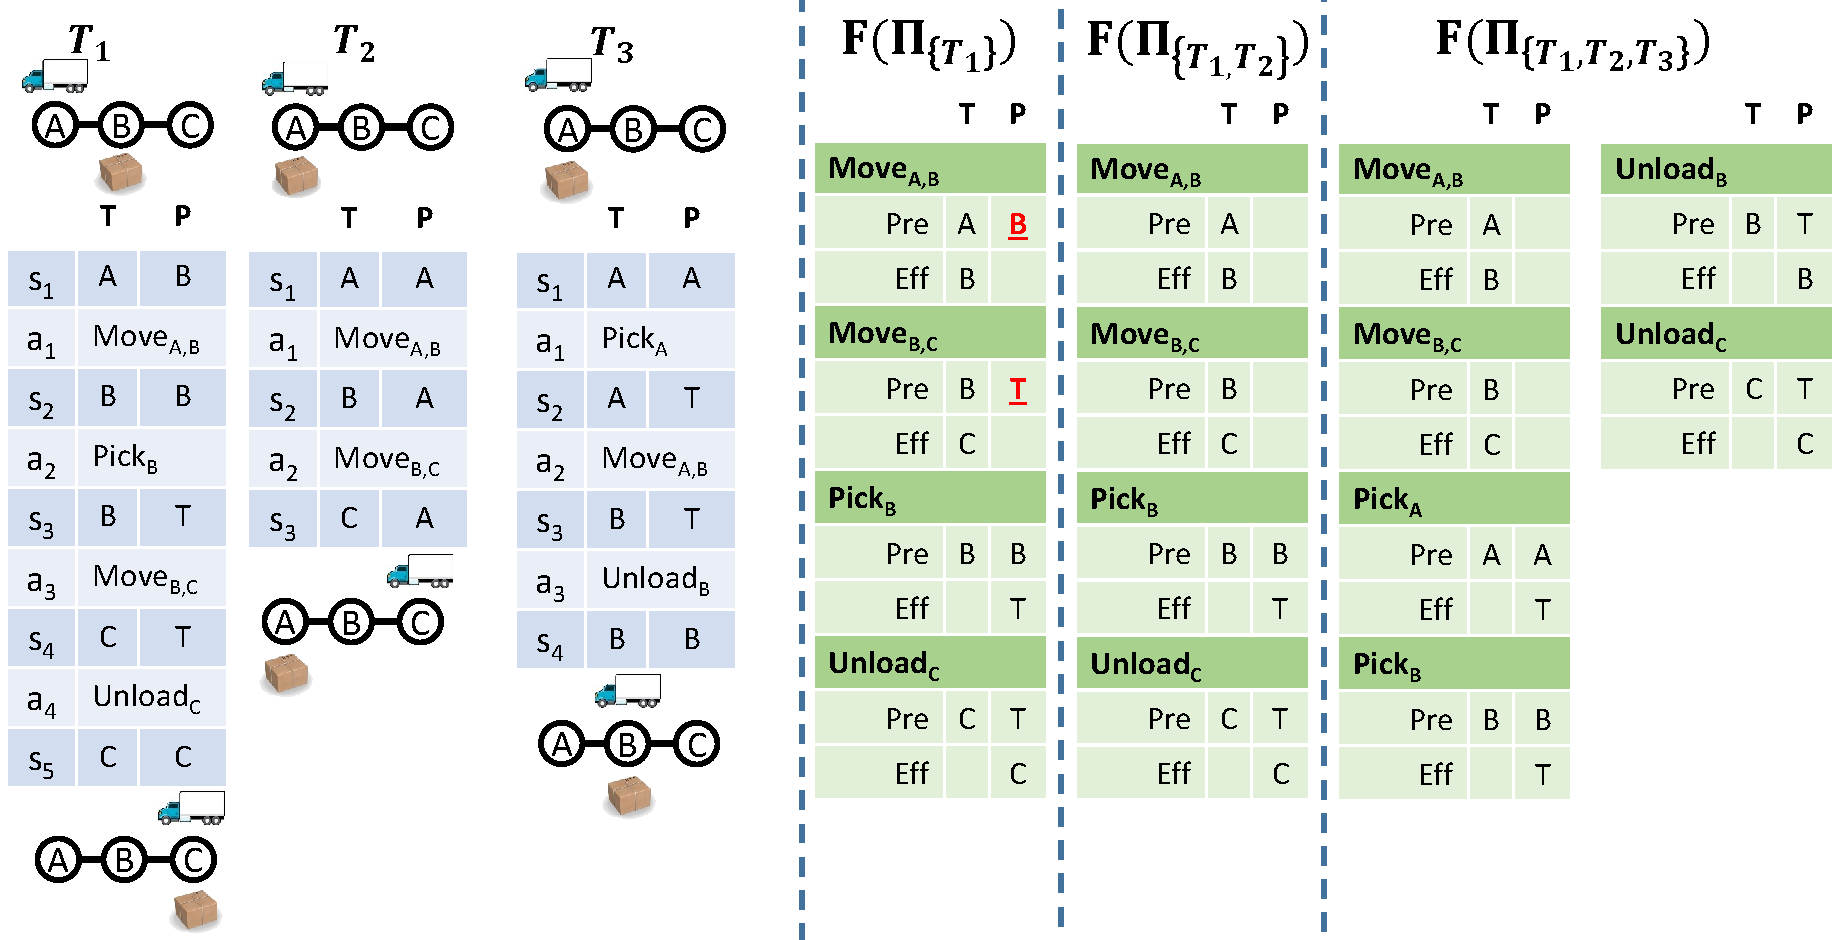
\includegraphics[width=\textwidth]{example_cropped.pdf}
	\caption{An example of creating $F(\Pi_{\mathcal{T}})$ from observed trajectories in a simple logistics-like domain. The left-hand side of the figure shows the three given trajectories $T_1$, $T_2$, and $T_3$. The right hand side of the figure shows our conservative action model, 
		learned using different subsets of the trajectories $T_1$, $T_2$, and $T_3$ together.}
	\label{fig:example}
	\end{figure*}
	
	
	
	Figure~\ref{fig:example} illustrates how to generate  $F(\Pi_{\mathcal{T}})$ from observed trajectories in a simple logistic-like domain with one truck, one package, and three possible location $A$, $B$, and $C$. The state variables are TruckAt, with domain $A$, $B$, and $C$, and PackageAt with domain $A$, $B$, $C$, and $T$, where $T$ represents that the package is on the truck. The possible actions are Move$_{X,Y}$, 
	Pickup$_X$, and Unload$_X$, for every $X,Y\in \{A,B,C\}$. 
	
	
	
	The three tables on the left-hand side, $T_1$, $T_2$, and $T_3$ are three observed trajectories, where the column $T$ represents the value of the state variable TruckAt and the column $P$ represents the value of the state variable PackageAt. For example, $T_1$ represents a trajectory where the truck starts at $A$, moves to $B$, picks up the package, moves to $C$, and unloads the package there. 	The tables on the right-hand side of Figure~\ref{fig:example} show the action model learned from these trajectories. For didactic reasons, we show the action model learned given just $T_1$ ($F(\Pi_{\{T_1\}})$), 
	then the action model learned given $T_1$ and $T_2$ ($F(\Pi_{\{T_1, T_2\}})$), and finally 
	the action model learned using all three trajectories. 
	
	
	As can be observed, given only $T_1$ we do not have any knowledge of many actions such as Pick$_A$, Pick$_C$, etc. Also, the preconditions learned for the actions Move$_{A,B}$ 
	and Move$_{B,C}$ are too restrictive, requiring that the package is at some location (while clearly a Move action only requires knowing the truck's location). However, given $T_1$ and $T_2$, these redundant preconditions are removed, and thus task that can be achieved with the actions Move$_{A,B}$, Move$_{B,C}$, Pick$_B$, and Unload$_C$ will be found by our conservative model-free planner. 
	
	
	
	\section{Learning to Perform Model-Free Planning}
	%[[Something about the impracticality of the solution above, and how we aim for a more general task, in which we want to maximize probability of success]]
	In general, we cannot guarantee that {\em any finite number of trajectories} will suffice to obtain {\em precisely} the underlying action model. This is because, for example, if some action never appears in a trajectory, we may not know its effects; or, if an action is only used in a limited variety of states, it may be impossible to distinguish its preconditions. Consequently, we cannot guarantee a complete solution to the conformant model-free planning problem. However, as the number of trajectories increases, we can hope to learn enough of the actions accurately enough to be able to find plans for most goals in practice. This gives raise to a statistical view of the conformant model-free planning task (Definition~\ref{def:model-free-planning}) that follows the usual statistical view of learning, along the lines of Vapnik and Chervonenkis~\shortcite{vapnik1971} and Valiant~\shortcite{valiant1984}.  %is:
	%In this work, we follow the usual statistical view of learning, along the lines of Vapnik and Chervonenkis~\shortcite{vapnik1971} and Valiant~\shortcite{valiant1984}. The main task we consider is:
	
	\begin{definition}[Conformant Model-Free Learning-to-Plan] We suppose that there is an arbitrary, unknown (prior) probability distribution $D$ over triples of the form $\tuple{I,s_\mathcal{I}, s_\mathcal{G}}$, where $s_\mathcal{I}$ is a state, $s_\mathcal{G}$ is a goal condition, and $T$ is a trajectory that starts in $s_\mathcal{I}$ and ends in a state that satisfies $s_\mathcal{G}$, 
		and all trajectories are applicable in a fixed planning domain $\mathcal{D}=\tuple{P,A}$. 
		%defined for a set of propositions $P$ and set of actions $A$ with a fixed action model. 
		In the conformant model-free learning-to-plan task, we are given a set of triplets $\tuple{s_\mathcal{I}^{(1)},s_\mathcal{G}^{(1)},T^{(1)}},\ldots,\tuple{s_\mathcal{I}^{(m)},s_\mathcal{G}^{(m)},T^{(m)}}$ drawn independently from $D$, 
		and a new \SAS{} planning problem $\Pi=\tuple{\mathcal{D}, s_\mathcal{I}, s_\mathcal{G}}$  
		such that the initial state and goal condition $(s_\mathcal{I},G)$ are from some $(s_\mathcal{I},s_\mathcal{G},T)$ drawn from $D$. 
		%The task is to either to output a plan for $\Pi$ or, with probability at most $\epsilon$, assert that no plan can be found.
		The task is to either output a plan for $\Pi$ or, with probability at most $\epsilon$, return that no plan was found.
		%In the model-free planning task, $(I^{(1)},G^{(1)},T^{(1)}),\ldots,(I^{(m)},G^{(m)},T^{(m)})$ have been drawn independently from $D$, and we are given as input $T^{(1)},\ldots,T^{(m)}$, and a new initial state and goal $(I,G)$ for some $(I,G,T)$ drawn from $D$. We must either output a plan for $\langle P,A,I,G\rangle$ or, with probability at most $\epsilon$, assert that no plan can be found.
		\label{def:learning-to-plan}
	\end{definition}
	
	
	
	%\MEMO{Roni: I think that since $I$ and $G$ are drawn from some $(I,G,T)$ drawn from $D$ then $(I,G)$ must be a solveable instance. So we should say that the learned action model is sufficient to generate a solution for  the planning problem $(I,G)$ with probability at least $1-\epsilon$. I don't think we can say something about the probability that the problem is not solvable  as we did not have cases like that in the training set  and having such cases means the traninig set used a different  distribution than reality}
	%\MEMO{Roni: Do we really need the distribution of $(I,G,T)$  and cannot assume only a distribution of ($I,G$)?  I think it will be cleaner to only talk about $D$ inthe proof of Theorem 1  and don't have it in the definition or theorem.}
	We stress that $D$ is arbitrary, and in particular the conditional distribution
	of trajectories given a start and goal state, $D(T|I,G)$, is completely 
	arbitrary. Even if $D(T|I,G)$ produces a deterministic outcome $T(I,G)$, this
	still captures, for example, the distribution of trajectories obtained
	by running some (unknown, sophisticated) planning algorithm on input $(I,G)$.
	It also captures a nondeterministic, adversarial choice of trajectory $T(I,G)$ to 
	be paired with the start state $I$ and goal $G$. 
	%We note that this task is conservative in the sense that when an algorithm solving it outputs a plan, the plan is required to be correct. The algorithm may only make errors by failing to find a plan when one exists. %\section{Theoretical Guarantees and Limitations} How many trajectories do we need to guarantee that every plan can be generated?
	A key question is how our certainty that a plan can be generated for a new start and goal state grows with the number of trajectories. Let $\log$ and $\ln$ denote $\log_2$ and $\log_e$, respectively, and let $d$ denote the largest number of values
	for a state variable. 
	%Since there are $n$ state variables each with at most $d$ values, 
	\begin{theorem}
		Using the conservative model-free planner, 
		it is sufficient to observe 
		%$m>\frac{(2ln 2)|A|}{\epsilon}(|P|+\log |A|+\log\frac{2}{\delta})$
		$m\geq\frac{(2\ln  d)|A|}{\epsilon}(n+\log\frac{2|A|}{\delta})$
		trajectories to solve the conformant model-free learning-to-plan problem with probability $1-\delta$. 
		\label{the:pac-conformant}
	\end{theorem}
	%\begin{proof}
	%\MEMO{Question \#1: There is a conceptual hop that I am missing. I understand that there is a distribution of start-goal pairs. But I don't understand the meaning of a distribution over trajectories. A trajectory is not something that follows some distribution, it is something that is computed by some planning process.}
	\begin{proof}
		{\bf Outline.} First, Lemma~\ref{lem:sufficientActions} shows 
		that the set of actions used by our conservative model-free planner ($A(\mathcal{T})$) 
		is sufficient to solve a randomly drawn problem with high probability. 
		Then, Lemma~\ref{lem:plan-existance} shows that 
		under certain conditions, the preconditions we learned for these actions ($\pre_\mathcal{L}^U$) 
		are not too conservative, i.e., they are adequate
		for finding a plan with high probability.  
		Finally, we prove that with high probability these conditions over the action model we learned 
		indeed hold. 
		
		
		% (Lemma~\ref{lem:sufficientActions}). Then, we show that under some conditions over the action model we learn is sufficient (i.e., they are not too conservative)t o enable finding a plan with high probability (Lemma~\ref{lem:plan-existance}). Finally, we show that these conditions indeed hold when using  conservative model-free planning. %although the set of preconditions we assume is conservative, it is still sufficient to enable finding a plan with high probability. 
		
		\begin{lemma}
			Let $A_\epsilon$ be the set of actions such that each action $a\in A_\epsilon$ appears in a trajectory sampled from $D$ with probability at least $\frac{\epsilon}{2|A|}$ and let $A(\mathcal{T})$ be the set of every action that appeared in a trace. 
			The probability that all the actions $a\in A_\epsilon$ 
			appear in $A(\mathcal{T})$ is at least $1-\delta/2$.
			%The probability that any action $a\in A_\epsilon$ does not appear in $A(\mathcal{T})$ is at most $\delta/2$.
			\label{lem:sufficientActions}
		\end{lemma}
		\begin{proof}
			By definition, the probability that an action $a\in A_\epsilon$ does not exist in a trajectory drawn from $D$ is $1-\frac{\epsilon}{2|A|}$. 
			Since the observed trajectories $\mathcal{T}$ are drawn independently from $D$ we have that the probability that $a\notin A(\mathcal{T})$ is
			$(1-\frac{\epsilon}{2|A|})^m\leq e^{-\frac{\epsilon\cdot m}{2|A|}}$, 
			using the inequality $1-x\leq e^{-x}$. 
			Since we assume in Theorem~\ref{the:pac-conformant} that $m>\frac{(2ln 2)|A|}{\epsilon}(n+\log |A|+\log\frac{2}{\delta})$
			which is larger than $\frac{(2\ln 2)|A|}{\epsilon}\log\frac{2|A|}{\delta}$, 
			we have that the probability that $a\notin A(\mathcal{T})$ is at most 
			\begin{equation}
			e^{-\frac{\epsilon\cdot m}{2|A|}}
			\leq e^{-\frac{\epsilon}{2|A|} \cdot \frac{(2\ln 2)|A|}{\epsilon}\log\frac{2|A|}{\delta}}
			=e^{-\ln\frac{2|A|}{\delta}}=\frac{\delta}{2|A|}
			\end{equation}
			Hence, by a union bound over $a\in A_\epsilon$ (noting $|A_\epsilon|\leq |A|$), we have that $A_\epsilon\subseteq A(\mathcal{T})$ with probability $1-\delta/2$ as needed.
		\end{proof}
		
		Stated informally, Lemma~\ref{lem:sufficientActions} says that with high probability we will observe
		all the ``useful'' actions, i.e., the actions used in many trajectories. However, we may have learned 
		preconditions for these actions that are too conservative, 
		preventing the planner from finding a plan even if one exists. 
		The next definition defines an action model property that states that this does not occur frequently. 
		
		% the execution of actions in states where they in fact can be executed. Due to Theorem~\ref{the:safeness} we know that observed actions will be associated with a safe action model. Still, the preconditions learned for the observed actions may be too restrictive, i.e., prevent the execution of actions in states where they in fact can be executed. 
		
		\begin{definition}[Adequate]
			We call an action model {\em $\epsilon$-adequate} if, with probability at most $\epsilon/2$, we sample a trajectory $T$ from $D$ such that $T$ contains an action triplet $\tuple{s,a,s'}$  where $a\in A_\epsilon$ and $s$ does not satisfy $\pre_\mathcal{T}^U$. 
			%We call an action model {\em inadequate} if, with probability at least $\epsilon/2$  we sample a trajectory $T$ from $D$ such that $T$ contains an action triplet $\tuple{s,a,s'}$  where $a\in A_\epsilon$ and $s\nsubseteq\pre_\mathcal{T}^U$. 
			\label{def:adequate}
		\end{definition}
		We say that an action model is {\em $\epsilon$-inadequate} if it is not $\epsilon$-adequate. 
		An equivalent way to define the notion of an {\em $\epsilon$-adequate} action model is
		that with probability at most $\epsilon/2$ 
		a trajectory is sampled in which an action $a\in A_\epsilon$ is invoked on a state that 
		does not satisfy the conservative preconditions of $a$ we learned from the given set of trajectories ($\mathcal{T}$).  
		
		
		\begin{lemma}
			If the learned action model is $\epsilon$-adequate and $A_\epsilon\subseteq A(\mathcal{T})$, 
			then with probability $1-\epsilon$ our conservative model-free planner will find a plan for a start-goal pair $(s_\mathcal{I},s_\mathcal{G})$ sampled from $D$.
			\label{lem:plan-existance}
		\end{lemma}
		\begin{proof}
			Let $T$ be the (unknown) trajectory sampled for $(s_\mathcal{I},s_\mathcal{G})$. 
			The probability that $T$ uses an action that is not in 
			$A_\epsilon$ is at most $|A|\cdot\frac{\epsilon}{2|A|}=\epsilon/2$. 
			Thus, $T$ contains only actions known to our planner with probability at least $1-\epsilon/2$, since we assumed that $A_\epsilon\subseteq A(\mathcal{T})$. 
			Since the action model is $\epsilon$-adequate then with probability $1-\epsilon/2$ the learned preconditions are satisfied on all of the states in $T$. Thus, by a union bound, we find that with probability $1-\epsilon$, our planner could at least find $\mathcal{T}$. Hence it will find a trajectory from $s_\mathcal{I}$ to $s_\mathcal{G}$, as required. 
		\end{proof}
		
		
		%In Theorem~\ref{the:safeness} we established that the action model used by our conservative model-free planner is safe. 
		Finally, we argue that the action model used by our conservative model-free planner is $\epsilon$-adequate with probability at least $1-\delta/2$. 
		Whether an action model is $\epsilon$-adequate or not depends on the assignment of preconditions to actions. 
		Since there are $n$ state variables each with at most $d$ values, 
		then there are $d^n$ possible assignments of preconditions for an individual action
		and a total of $d^{n\cdot |A|}$ possible preconditions assignments for an action model . 
		Let $BAD$ be the subset of these action model preconditions assignments that are not $\epsilon$-adequate. 
		Clearly, $BAD$ has size of at most $d^{n\cdot |A|}$. 
		
		
		Consider a particular assignment of preconditions in an $\epsilon$-inadequate action model $\mathcal{O}_{BAD}$. Since $\mathcal{O}_{BAD}$ is $\epsilon$-inadequate, 
		it has a set of state-action pairs ($s,a$) associated with it such that $a\in A_\epsilon$ and $a$ cannot be applied to $s$ according to $\mathcal{O}_{BAD}$. 
		The action model $\mathcal{O}_{BAD}$ can only be learned by our algorithm 
		if none of these state-action pairs were observed in the given trajectories $\mathcal{T}$. 
		On the other hand, by the definition of inadequacy
		the probability of having a state-action pair from that list 
		in a trajectory drawn from $D$ is at least $\epsilon/2$. 
		Thus, the probability that our algorithm will learn a particular preconditions assignment of an $\epsilon$-inadequate action model is at most $(1-\epsilon/2)^m$.
		Since $m\geq\frac{(2\ln  d)|A|}{\epsilon}(n+\log\frac{2|A|}{\delta})>\frac{2\ln d}{\epsilon}(|A|\cdot n+\log\frac{2}{\delta})$, then $(1-\epsilon/2)^m$ is smaller than 
		
		%\begin{equation}
		%e^{-\frac{\epsilon}{2} \cdot m}\leq 
		%e^{-(\ln 2 \cdot (|A||P|+\log\frac{2}{\delta}))}
		%=e^{-\ln 2 \cdot |A||P|}\cdot e^{-\ln  \frac{2}{\delta}}=\frac{\delta}{2^{|A||P|}}
		%\leq e^{-\frac{\epsilon}{2|A|} \cdot \frac{(2\ln 2)|A|}{\epsilon}\log\frac{2|A|}{\delta}}
		%=e^{-\ln\frac{2|A|}{\delta}}=\frac{\delta}{2|A|}
		%\end{equation}
		
		
		\begin{equation}
		e^{-\frac{\epsilon}{2} \cdot m}
		\leq 
		e^{-(\ln d \cdot (|A|\cdot n+\log\frac{2}{\delta}))}
		=e^{-\ln d \cdot |A|\cdot n}\cdot e^{-\ln  \frac{2}{\delta}}
		%=\frac{\delta}{d^{n\cdot |A|}}
		\end{equation}
		which is at most $\delta/d^{n\cdot |A|}$. Thus, by a union bound over this set of inadequate assignments $BAD$, the probability that any inadequate assignment of preconditions could be output is at most $\delta/2$.
		%We finally note that the algorithm cannot produce unsafe preconditions for $A(\mathcal{T})$: indeed, observe that the preconditions are satisfied for every action invoked in every trajectory obtained by the algorithm. Since the algorithm includes all of the literals that are satisfied on all of the states in which that action was invoked, in particular it includes all of the literals that actually appear in the precondition. 
		Thus, with probability $1-\delta$, the algorithm indeed produces an assignment of preconditions that is neither unsafe for $A(\mathcal{T})$ nor inadequate for $A_\epsilon$, as needed.
	\end{proof}
	
	\subsection{Unsolvable Instances}
	
	The implication of Theorem~\ref{the:pac-conformant} is that by observing 
	a number of trajectories that is linear in the number of actions and the number of state variables, 
	we expect our conformant model-free planner to be complete with high probability, in the sense that if a solution exists it will be found. But what if some of the drawn problem instances are not solvable? 

\begin{table}
	\centering
	\begin{tabular}{c|c|c|c}
			& $\plannable (\Pi)$ & $\neg\plannable(\Pi)$ & Priors \\ \hline
		$\solvable(\Pi)$ 		& $1-\epsilon$ & $\epsilon$ & $\mu$ \\
		$\neg\solvable(\Pi)$	& 0 & 1 & $1-\mu$ \\ \hline
		Marginals	& $\mu (1-\epsilon)$ & $1-\mu(1-\epsilon)$ &
	\end{tabular}
\caption{The table shows the priors, conditional probabilities, and marginals obtained with probability $1-\delta$ when using our conservative model-free planner when it is given $m\geq\frac{(2\ln  d)|A|}{\epsilon}(n+\log\frac{2|A|}{\delta})$ trajectories.}
\label{tab:probabilities}	
\end{table}

	\begin{corollary}
		If the probability of drawing a solvable start-goal pair from $D$ is $\mu$ then it is sufficient to 
		observe $m\geq\frac{(2\ln  d)|A|}{\epsilon}(n+\log\frac{2|A|}{\delta})$
		trajectories (of solvable instances) to guarantee that with probability of at least $1-\delta$ our conservative model-free planner will solve a start-goal pair drawn from $D$ with probability at least $\mu\cdot(1-\epsilon)$ 
\label{cor:unsolvable}
	\end{corollary}
\begin{proof}
	Let $\solvable(\Pi)$ be true or false if  a given planning problem $\Pi$ is solvable or unsolvable, respectively, 
	and let $\plannable(\Pi)$ be true or false if our planner returns a solution to $\Pi$ or not respectively. We aim to bound $Pr(\plannable(\Pi))$. Since our planner is sound, $\plannable(\Pi)\rightarrow \solvable(\Pi)$ and so
	\[ Pr(\plannable(\Pi))= Pr(\plannable(\Pi)\wedge \solvable(\Pi))= Pr(\plannable(\Pi)|\solvable(\Pi))\cdot Pr(\solvable(\Pi)) \]
	According to Theorem~\ref{the:pac-conformant}, 
	$Pr(\plannable(\Pi)|\solvable(\Pi))\geq 1-\epsilon$ 
	and $Pr(\solvable(\Pi))=\mu$ by definition. 
\end{proof}

Table~\ref{tab:probabilities} shows the priors, conditional probabilities, and marginals use by the proof of Corollary~\ref{cor:unsolvable}
The first row shows the probabilities 
	$Pr(\plannable(\Pi)|\solvable(\Pi))$, 
	$Pr(\neg\plannable(\Pi)|\solvable(\Pi))$, abd
	$Pr(\solvable(\Pi))$; 
	the second row shows the probabilities 
	$Pr(\plannable(\Pi)|\neg\solvable(\Pi))$, 
	$Pr(\neg\plannable(\Pi)|\neg\solvable(\Pi))$, and
	$Pr(\neg\solvable(\Pi))$;  	
	and the last row shows the marginal probabilities
	$Pr(\plannable(\Pi))$ and  
	$Pr(\neg\plannable(\Pi))$. 
	
	Corollary~\ref{cor:unsolvable} and Table~\ref{tab:probabilities} are valuable in that they provides a relationship between $\mu$, $\epsilon$, $\delta$, and $m$. Thus, we can increase $m$ to satisfy more demanding values of $\mu$, $\epsilon$, and $\delta$ and different types of error bounds. For example, consider an application that requires bounding, by some $\gamma$, the probability that our planner outputs incorrectly that no plan exists. In other words, an application that requires 
	\[ Pr(\solvable(\Pi)|\neg\plannable(\Pi))\leq \gamma \]
	Using Bayes rule and the values from Table~\ref{tab:probabilities}, this means that 
	\[ \frac{\epsilon\cdot\mu}{1-(1-\epsilon)\cdot\mu}\leq \gamma \Leftrightarrow  \epsilon\leq \frac{\gamma\cdot (1-\mu)}{\mu\cdot (1+\gamma)}\]
	\noindent Plugging $\frac{\gamma\cdot (1-\mu)}{\mu\cdot (1+\gamma)}$ into the sample complexity instead of $\epsilon$ in Theorem~\ref{the:pac-conformant} will give the required number of trajectories to obtain a bound of  $\gamma$ on the probability of incorrectly outputting that a problem is not solvable. 
	
	\subsection{Limited Planner Capabilities}
	The given trajectories $\mathcal{T}$ are presumably generated by some planning entity. Since planning in general is a hard problem, it may be the case that the planner that generated the given set of trajectories has drawn a solvable problem from $D$ but was just not able to solve it due to memory or time constraints. 
	
	Learning from such a set of trajectories does not enable bounding the probability of solving problems in general. What can be obtained in such cases is to bound the solving capabilities of our conservative model-free planner with respect to the capabilities of the planner that generated the observed trajectories. Thus, instead of having $\mu$ represent the probability that an instance is solvable, we will have $\mu$ represent the probability that an instance is solvable by the original planner. The rest of the analysis follows exactly the same as in the previous section.
	
	
	\section{Related Work}
	%This work focuses on a simpler setting in which there is full state observability, actions have deterministic effects, and there are no conditional effects. Jim{\'e}nez et al.~\shortcite{jimenez2012review} review the state-of-the-art in learning action models for this setting and other more complex settings (partial observability and non-deterministic action outcomes).
	
	Our work relates to several well-studied types of problems: planning under uncertainty, reinforcement learning, and domain modeling. 
	Unlike common planning under uncertainty models such as MDPs and POMDPs, our uncertainty does not 
	stem from the stochastic nature of the world or imperfect sensors, but from  not knowing the action model of the underlying planning problem. Unlike reinforcement learning, our task is to generate a plan that {\em must} work, and thus cannot rely on a trial-and-error approach to learn the domain and/or how to plan in it. 
	Similarly, most prior work on learning a domain model in general or a STRIPS action model from observed trajectories, also involve some form of trial-and-error as well, interacting with environment to refine the learned model~\cite{mourao2012learning,wang1994learning,wang1994learning,walsh2008efficientLearning,levine2006explanation,jimenez2013integrating}. 
	
	%DeJong~\shortcite{levine2006explanation} showed how to learn control operators  from background knowledge and experimentations. Jim{\'e}nez et al.~\shortcite{jimenez2013integrating} also studied how to integrate learning of planning operators and planning, including experimenting with planning rules that are probably correct Others interleaved planning and experimentation to 
	
	While we build on ideas from these prior works, our work is significantly different, as we demand that  the plan generated by the learned model {\em must} reach the goal, thus not allowing any form of trial-and-error. 
	%While trial-and-error is a reasonable approach in some cases, especially if the agent can re-plan during execution, it is unacceptable in other cases, e.g., when failure corresponds to physical harm to the acting agent or the agent has no re-planning capabilities.  
	In addition, most works learn from both positive and negative examples -- observing successful and failed trajectories, while we only require successful trajectories to be provided. 
	Another key difference is that unlike our work, most prior works do not provide statistical guarantees on the soundness of the plan generated with their learned model. 
	
	
	%{\em must} work, while all the works above allowed the generated plan to fail (possibly learning new information from such failures). Plan failures may be acceptable in some cases if the agent can re-plan during execution, but is unacceptable in other cases, e.g., where failure corresponds to physical harm to the acting agent. 
	
	% approach similar to reinforcment learning. Mour{\~{a}}o et al.~\shortcite{mourao2012learning} learned a STRIPS action model from from observed trajectories by using Machine Learning to predict whether an action is applicable and what are its effects. Levine and DeJong~\shortcite{levine2006explanation} showed how to learn control operators  from background knowledge and experimentations. Jim{\'e}nez et al.~\shortcite{jimenez2013integrating} also studied how to integrate learning of planning operators and planning, including experimenting with planning rules that are probably correct. Wang~\shortcite{wang1995learning,wang1994learning} proposed a process for learning a STRIPS model that includes learning an action model. She also discussed how to refine that action model by interacting with the world. 
	%While we build on ideas from these prior work, our task is fundamentally different, in that we do not allow experimentation or interleaving of planning and execution, and aim for a plan that is guaranteed to be sound.
	%A similar approach is taken in many reinforcement learning algorithms. Again, our task is different, in that we do not allow experimentation and aim for a plan that is guaranteed to be sound. Jim{\'e}nez et al.~\shortcite{jimenez2013integrating} also studied how to integrate learning of planning operators and planning. Their approach included an option to experiment with planning rules that are probably correct, while we aim for a provably sound plan. 
	%Walsh and Littman~\shortcite{walsh2008efficientLearning} discuss the problem of learning STRIPS operators from observed trajectories. They too interleave planning and execution: they learn an action model, find a plan for a given planning problem, and update that action model by the success or failure of the generated plan. 
	
	An exception to this is the work of Walsh and Littman~\shortcite{walsh2008efficientLearning}, that also discussed the problem of learning STRIPS operators from observed trajectories and provided theoretical bounds on the sample complexity -- the number of interactions that may fail until the resulting planner is  sound and complete.  By contrast, we do not assume any planning and execution loop and do not allow failed interactions. Hence, we aim for a planning algorithm that is guaranteed to be sound, at the cost of completeness. This difference affects their approach to learning. They attempted to follow an optimistic assumption about the preconditions and effects of the learned actions, in an effort to identify inaccuracies in their action model. By contrast, we are forced to take a pessimistic approach, as we aim for a successful execution of the plan rather than information gathering to improve the action model. 
	
	%. They proposed a planning and learning approach for learning STRIPS operators 
	%. Moreover, a key requirement in our work is that the plan generated by the learned actions {\em must} work, while all the works above allowed the generated plan to fail (possibly learning new information from such failures). Plan failures may be acceptable in some cases if the agent can re-plan during execution, but is unacceptable in other cases, e.g., where failure corresponds to physical harm to the acting agent. 
	%Walsh and Littman~\shortcite{walsh2008efficientLearning} also discuss the problem of learning STRIPS operators from observed trajectories. They too interleave planning and execution: they learn an action model, find a plan for a given planning problem, and update that action model by the success or failure of the generated plan. 
	%Unlike other work, they also provide a theoretical bounds on the sample complexity -- the number of interactions needed in order to guarantee that the resulting planner is sound and complete. By contrast, we do not assume any planning and execution loop, and we aim for a planning algorithm that is guaranteed to be sound, at the cost of completeness. 
	%This affects their approach to learning: they attempted to follow an optimistic assumption about the preconditions and effects of the learned actions, in an effort to identify inaccuracies in their action model. By contrast, we are forced to take a pessimistic approach, as we aim for a successful execution of the plan rather than information gathering to improve the action model. 
	%Unlike our work, she discussed how to refine that action model by interacting with the world, including learning from failed executions of actions.  We require that the plan generated by the learned actions {\em must} work. This is suitable for setting where plan failure is unacceptable, e.g., where failure corresponds to physical harm to the acting agent. 
	
	%addressed the problem of learning STRIPS actions given a set of observed trajectories. In their setting, the observed trajectories consist of cases in which the agent tried to perform an action and failed, while in our case the observations are only successful trajectories. Also, we assume full observability while they considered partial and noisy observations of the states in the trajectories. Their approach was to use machine learning methods to predict the outcome of an action and to predict whether it is applicable. Consequently, the plan generated by using this model can fail. By contrast, we aim for a plan that is guaranteed to work. Another similarity of this paper to the paper Mour{\~{a}}o et al.~\shortcite{mourao2012learning} 
	
	%The most related type of planning under uncertainty model is fully obserable non-deterministic planning in general and conformant planning in particular, as discussed and 
	%Our uncertainty stems from not knowing the action model, while algorithms for planning under uncertainty often accept as input the uncertainty  encoded in the problem description, e.g., ch is different from planning under uncertainty proms several lines of work. On the one hand, work on planning under various types of uncertainty has been widely studied in the planning literature. Highly related is the work on conformant planning~\cite{} and full observability non-determinisitc (FOND) planning~\cite{}. A key difference is we do not have the agent's action model and must learn how they agent acts from trajectories.  , 
	
	%Mour{\~{a}}o et al.~\shortcite{mourao2012learning} addressed the problem of learning STRIPS actions given a set of observed trajectories. In their setting, the observed trajectories consist of cases in which the agent tried to perform an action and failed, while in our case the observations are only successful trajectories. Also, we assume full observability while they considered partial and noisy observations of the states in the trajectories. Their approach was to use machine learning methods to predict the outcome of an action and to predict whether it is applicable. Consequently, the plan generated by using this model can fail. By contrast, we aim for a plan that is guaranteed to work. Another similarity of this paper to the paper Mour{\~{a}}o et al.~\shortcite{mourao2012learning} 
	
	%Also related is the work of Konidaris et al.~\shortcite{konidaris2014constructing} who showed how to learn a STRIPS model that provides a useful high-level plan for a continuous world. 
	
	
	%The aforementioned work of Wang~\shortcite{wang1995learning,wang1994learning} is, of course, very related to our work. She proposed a process for learning a STRIPS model that includes learning an action model. Unlike our work, she discussed how to refine that action model by interacting with the world, including learning from failed executions of actions.  We require that the plan generated by the learned actions {\em must} work. This is suitable for setting where plan failure is unacceptable, e.g., where failure corresponds to physical harm to the acting agent.  
	
	
	%Walsh and Littman~\shortcite{walsh2008efficientLearning} also discuss the problem of learning STRIPS operators from observed trajectories. They too interleave planning and execution: they learn an action model, find a plan for a given planning problem, and update that action model by the success or failure of the generated plan. 
	
	
	
	\section{Conclusions}
	This paper deals with a planning problem in which the planner agent has no knowledge about its actions. Instead of an action model, the planner is given a set of observed trajectories of successfully executed plans. 	In this setting we introduced the {\em conformant model-free planning} problem, in which the task is to find a plan that is guaranteed to reach the goal, i.e., there is no tolerance for execution failure. This type of problem is important in cases where failure is costly or in cases where the agent has no capability to replan during execution. 
	We showed how to use the given set of trajectories to learn
	about the agent's actions, bounding the set of predicates in the actions'  preconditions and effects. Then, we proposed a conservative approach to solve the conformant model-free problem that is based on a translation to a classical planning problem. This solution is sound but is not complete, as it may fail to find a solution even if one exists. However, we prove that under some assumptions the likelihood of finding a solution with this approach grows linearly with the number of predicates and quasi-linearly with the number of actions. 
	
	
	Future directions for conformant model-free planning include studying how to consider richer underlying planning models including parametrized actions, conditional effects, stochastic action outcomes, and partial observability. While some of these more complex action models can be compiled away (e.g., a problem with conditional effects can be compiled to a problem without conditional effects~\cite{nebel2000compilability}), the resulting problem can be significantly larger.   
	
	
	%Another future direction will consider cases where the given planning problem is not solvable.
	%Note that we cannot distinguish between cases where our planner outputted that no solution has been found from cases where indeed there are no solution. Future work can study and analyze the probability of such cases.
	
	%% The file named.bst is a bibliography style file for BibTeX 0.99c
	\bibliographystyle{named}
	\bibliography{library}
	
\end{document}

